	%!TEX root = ../thesis.tex
%*******************************************************************************
%*********************************** Theory chapter *****************************
%*******************************************************************************

\chapter{Theory}

\ifpdf
    \graphicspath{{chapter-theory/Figs/Raster/}{chapter-theory/Figs/PDF/}{chapter-theory/Figs/}}
\else
    \graphicspath{{chapter-theory/Figs/Vector/}{chapter-theory/Figs/}}
\fi

This chapter starts with an outline of the basic principles and concepts of the Standard Model of Particle Physics (SM), the theoretical framework describing nature on the level of elementary particles. This is followed by an introduction to supersymmetry, a promising class of theories aiming to solve some of the shortcomings of the SM.

By no means intended to be a full description, this chapter merely tries to highlight the important relations and consequences of the SM and supersymmetry. The mathematical description of this chapter largely follows~\cite{Brock:1354959, Peskin:1995ev} for the SM and~\cite{Martin:1997ns} for supersymmetry.

\section{The Standard Model of Particle Physics}

\nomenclature[z-SM]{SM}{Standard Model of Particle Physics}
\nomenclature[z-LEP]{LEP}{Large Electron Positron Collider}
\nomenclature[z-QED]{QED}{Quantum Electrodynamics}

By the end of the 1920s, quantum mechanics and general relativity had been relatively well established and the consensus among physicists was that matter was made of nuclear atoms consisting of electrons and protons. During the 1930s, a multitude of new experimental discoveries and theoretical puzzles excited physicists in three main fields of research: nuclear physics, cosmic rays and relativistic quantum mechanics. The following years and decades saw particle physics emerge as a result of these currents ultimately flowing together.

Since these early times of particle physics research, physicists have made extraordinary progress in describing nature at the subatomic scale. Today, a century later, the resulting theoretical framework, the Standard Model of Particle Physics, is the most fundamental theory of nature to date. It provides an extremely precise description of the interactions of elementary particles and---using the Large Electron Positron collider (LEP)---has been tested and verified to an unprecedented level of accuracy up to the electroweak (EWK) scale. Given the unprecedented success of SM, it is not surprising that its history is paved with numerous awards for both experimental and theoretical work. In 1964, the Nobel prize was awarded to Feynman, Schwinger and Tomonoga for their fundamental work in quantum electrodynamics (QED). This quantum field theory allows to precisely calculate fundamental processes as e.g. the anomalous magnetic moment of the electron to a relative experimental uncertainty of $2.3 \times 10^{-10}$~\cite{Mohr:2015ccw}. In 1979, Glashow, Weinberg and Salam were awarded with the Nobel prize for their work towards electroweak unification. The most prominent recent progress is undoubtedly the discovery of the Higgs boson, not only resulting in the Nobel prize being awarded to Englert and Higgs, but also completing the SM, roughly 50 years after the existence of the Higgs boson had been theorised. 

	\improvement{Couplings and masses are measured from experiment}
		
\subsection{Particle content of the SM}

\begin{table}
	\centering
	\setlength\heavyrulewidth{0.2ex}
	\small
	\caption{Names, electric charges and masses (rounded to three significant digits if known to that precision) of all observed fermions in the SM~\cite{pdg2020}.}
	\begin{tabular} {c c c c c}
		
		\toprule
				& generation & particle & electric charge [$e$] & mass \\ 
		\midrule 
				\multirow{6}{*}{leptons}& \multirow{2}{*}{1} & electron ($e$)& $-1$ & \SI{511}{\keV}\\
				& & electron neutrino ($\nu_e$) & 0 & < \SI{2}{\eV} \\
				& \multirow{2}{*}{2} & muon ($\mu$)& $-1$ & \SI{106}{\MeV}\\
				& & muon neutrino ($\nu_\mu$) & 0 & < \SI{0.19}{\MeV} \\
				& \multirow{2}{*}{3} & tau ($\tau$)& $-1$ & \SI{1.78}{\GeV}\\
				& & tau neutrino ($\nu_\tau$) & 0 & < \SI{18.2}{\MeV} \\
		\midrule 
				\multirow{6}{*}{quarks}& \multirow{2}{*}{1} & up ($u$)& $\frac{2}{3}$ & \SI{2.3}{\MeV}\\
				& & down ($d$) & $-\frac{1}{3}$ & \SI{4.8}{\MeV} \\
				& \multirow{2}{*}{2} & charm ($c$)& $\frac{2}{3}$ & \SI{1.28}{\GeV}\\
				& & strange ($s$) & $-\frac{1}{3}$ &\SI{95}{\MeV} \\
				& \multirow{2}{*}{3} & top ($t$)& $\frac{2}{3}$ & \SI{173}{\GeV}\\
				& & bottom ($b$) & $-\frac{1}{3}$ & \SI{4.18}{\GeV} \\
		\bottomrule
	\end{tabular}\vspace{3mm}
	\label{tab:particles_fermions}   
\end{table}

The SM successfully describes \change{Neutrino masses not in SM!} ordinary matter as well as their interactions, namely the electromagnetic, weak and strong interactions. Gravity is the only fundamental force not described within the SM. The particles in the SM are classified into two main categories, depending on their spin. Particles with half-integer spin follow Fermi-Dirac statistics and are called fermions. As they are subject to the Pauli exclusion principle, they make up ordinary matter. Particles with integer spin follow Bose-Einstein statistics and mediate the fundamental interactions between fermions. 

%\subsubsection*{Fermions} 

Fermions are further divided into leptons and quarks, which each come in three generations with increasing masses\footnote{Neutrinos might not exist in a normal mass hierarchy but could also have an inverted mass hierarchy.}. The three electrically charged leptons are each associated with a corresponding neutral neutrino (more on this \textit{association} in chapter\info{need ref}). While the SM assumes massless neutrinos, the observation of neutrino oscillations~\cite{Fukuda:1998mi} implies the existence of at least two massive neutrinos. By extending the SM to allow non-vanishing neutrino masses, neutrino oscillations can be introduced through lepton generation mixing, described by the Pontecorvo-Maki-Nakagawa-Sakata (PMNS)\nomenclature[z-PMNS]{PMNS}{Pontecorvo–Maki–Nakagawa–Sakata} matrix~\cite{PMNS:1962mu}. Apart from an electric charge, the six quarks also carry a colour charge. There are three types of colour charge: \textit{red}, \textit{green} and \textit{blue} as well as their respective anti-colours. The mixing in the quark sector through the weak interaction can be described by the Cabibbo-Kobayashi-Maskawa (CKM)\nomenclature[z-CKM]{CKM}{Cabibbo-Kobayashi-Maskawa} matrix~\cite{PhysRevLett.10.531,CKM:1973fv}. Finally, each fermion comes with its own anti-particle with same mass and spin, but inverted charge-like quantum numbers\footnote{The exact nature of anti-neutrinos is still an open question and ties into whether or not the neutrino mass matrix contains non-vanishing Majorana mass terms.}. All fermions in the SM are listed in \cref{tab:particles_fermions}.

%\subsubsection*{Bosons}

\begin{table}
	\centering
	\setlength\heavyrulewidth{0.2ex}
	\small
	\caption{Names, electric charges and masses (rounded to three significant digits if known to that precision) of all observed bosons in the SM~\cite{pdg2020}.}
	\begin{tabular} {c c c c}
	\toprule
		particle & spin & electric charge [$e$]& mass \\ 
	\midrule
		photon ($\gamma$) & 1 & 0 & 0\\
		gluon ($g$) & 1 & 0 & 0 \\
		$W^\pm$ & 1 & $\pm 1$ & \SI{80.4}{\GeV} \\
		$Z^0$ & 1 & 0 & \SI{91.2}{\GeV} \\
		Higgs boson ($H$) & 0 & 0 & \SI{125}{\GeV} \\
	\bottomrule					
	\end{tabular}\vspace{3mm}
	\label{tab:particles_bosons}   
\end{table}

The fundamental forces described by the SM are propagated by bosons with spin $1\hbar$. The photon $\gamma$ couples to electrically charged particles and mediates the electromagnetic interaction. As the photon is massless, the electromagnetic force has infinite range. The strong force is mediated by gluons carrying one unit of colour and one unit of anti-colour. Due to colour-confinement, colour charged particles like quarks and gluons cannot exist as free particles and instead will always form colour-neutral bound states. Although nine gluon states would theoretically be possible, only eight of them are realised in nature: the colour-singlet state $\frac{1}{\sqrt{3}}(\ket{r\bar{r}}+\ket{g\bar{g}}+\ket{b\bar{b}})$ would be colour-neutral result in long-range strong interactions, which have not been observed.\info{Might want to explain this later once I introduced the gauge groups?} Finally, the weak force is mediated by a total of three bosons, two charged $W$-bosons $W^+$ and $W^-$, and a neutral $Z$-boson. The mediators of the weak force are massive, resulting in a finitely ranged interaction. The $W^\pm$ and $Z$ bosons gain their masses through the Higgs mechanism (discussed in chapter \info{need ref}), resulting in a massive spin-0 boson, called the Higgs boson. All bosons known to the SM are listed in \cref{tab:particles_bosons}.


\subsection{The SM as a gauge theory}\label{ch:gauge_theory}

\nomenclature[z-QFT]{QFT}{Quantum Field Theory}
\nomenclature[z-QCD]{QCD}{Quantum Chromodynamics}

Formally, the SM is a collection of a special type of quantum field theories, called gauge theories. Quantum field theory (QFT) is the application of quantum mechanics to dynamical systems of fields, just as quantum mechanics is the quantisation of dynamical systems of particles. QFT provides a uniform description of quantum mechanical particles and classical fields, while including special relativity.

In classical mechanics, the fundamental quantity  is the action $S$, which is the time integral of the Lagrangian $L$, a functional characterising the state of a system of particles in terms of generalised coordinates $q_1, \dots, q_n$. In field theory, the Lagrangian can be written as spatial integral of a Lagrangian density $\Lagr(\phi_i,\partial_\mu\phi_i)$, that is a function of one or more fields $\phi_i$ and their spacetime derivates $\partial_\mu\phi_i$. For the action, this yields
\begin{equation}
	S = \int L\diff t = \int\Lagr\left(\phi_i,\partial_\mu\phi_i\right)\Diff4 x.
\end{equation}
In the following, the Lagrangian density $\Lagr$ will simply be referred to as the \textit{Lagrangian}.

Using the principle of least action $\delta S = 0$, the equation of motions for each field are given by the Euler-Lagrange-equation,
\begin{equation}
	\partial_\mu\left(\frac{\partial\Lagr}{\partial\left(\partial_\mu\phi_i\right)}\right)-\frac{\partial\Lagr}{\partial\phi_i}=0.
	\label{eq:euler_lagrange}
\end{equation}
As opposed to the Hamiltonian formalism, the Lagrange formulation of field theory is especially well suited in this context, as it exhibits explicit Lorentz-invariance. This is a direct consequence of the principle of least action, since boosted extrema in the action will still be extrema for Lorentz-invariant Lagrangians.

\improvement{Explicitly derive the Euler-Lagrange equations? Cf. Peskins Ch.2.2.}

Symmetries are of central importance in the SM. As Emmy Noether has famously shown in 1918~\cite{physics/0503066} for classical mechanics, every continuous symmetry of the action has a corresponding conservation law. In the context of classical field theory, each generator of a continuous internal or spacetime symmetry transformation leads to a conserved current, and thus to a conserved charge. In QFTs, quantum versions of Noether's theorem, called Ward–Takahashi identities~\cite{PhysRev.78.182,Takahashi1957} for Abelian theories and Slavnov–Taylor identities~\cite{THOOFT1971173,TAYLOR1971436,Slavnov1972} for non-Abelian theories relate the conservation of quantum currents and charge-like quantum numbers to continuous global symmetries of the Lagrangian.\unsure{Check correctness of formulation}

From a theoretical point of view, the SM can be described by a non-Abelian Yang-Mills type \improvement{cite YM} gauge theory based on the symmetry group
\begin{equation*}
	SU(3)_C \otimes SU(2)_L \otimes U(1)_Y,
\end{equation*}
where $U(n)$ ($SU(n)$) describes (special) unitary groups, \ie the Lie groups of $n\times n$ unitary matrices (with determinant 1, if special). $SU(3)_C$ generates quantum chromodynamics (QCD), \ie the interaction of particles with colour charge through exchange of gluons, and $SU(2)_L \otimes U(1)_Y$ generates the electroweak interaction. Here, the subscript $Y$ represents the weak hypercharge, while the $L$ indicates that $SU(2)_L$ only couples to left-handed particles (right-handed antiparticles).

\subsubsection{Feyman diagrams}

Transitioning from classic field theory to quantum field theory is typically done either through canonical quantisation or through the usage of path integral formalism. Only the the simplest field theories can be solved analytically, namely those containing only free fields, without any interactions. Perturbation theory has to be used for calculating scattering cross sections and decay rates for any QFT containing interactions. Any transition matrix can then be written as a series expansion in the coupling constant, with each term represented by a Feynman diagram. 

Using appropriate Feynman rules dictating the possible vertices (representing interactions between fields) and propagators (representing the propagation of fields), an infinite number of Feynman diagrams can be written down. Given the incoming and outgoing particles, all possible combinations of propagators and vertices that can be placed in between (\ie all possible Feynman diagrams) represent the full perturbation series. Only the lowest order in the series is considered at leading order (LO), the next-lowest at next-to-leading order (NLO), and so on. \unsure{is this paragraph correct?}


\subsubsection{Gauge principle}
\label{sec:gauge_principle}

The gauge principle is fundamental to the SM and dictates that the existence of gauge fields is directly related to symmetries under local gauge transformations. QED, being the simplest gauge theory, can be taken to illustrate this important principle. The free Dirac Lagrangian for a single, non-interacting fermion with mass $m$ is given by
\begin{equation}
	\Lagr_\mathrm{Dirac}=\bar{\psi}\left(i\gamma^\mu\partial_\mu - m\right)\psi,
	\label{eq:dirac_lagrangian}
\end{equation}
where $\psi$ is a four-component complex spinor field, $\bar{\psi} = \psi^\dagger\gamma^0$, and $\gamma^\mu$ with $\mu = 0,1,2,3 $ are the Dirac matrices with the usual anticommutation relations generating a matrix representation of the Dirac algebra 
\begin{equation}
	\{\gamma^\mu,\gamma^\nu\} \equiv \gamma^\mu\gamma^\nu + \gamma^\nu\gamma^\mu = 2\eta^{\mu\nu}\mathbb{1}_4.
\end{equation}

It is worth noting that the free Dirac Lagrangian is invariant under a global $U(1)$ transformation
\begin{equation}
	\psi \rightarrow e^{i\theta}\psi,
\end{equation}
where the phase $\theta$ is spacetime independent and real. In order to produce the physics of electromagnetism, the free Dirac Lagrangian however has to be invariant under \textit{local} $U(1)$ phase transformations, which is not the case, as the transformed Lagrangian picks up an additional term from the spacetime derivative of the phase $\partial_\mu\theta(x)$.

In order for the Dirac Lagrangian to become invariant under a local gauge transformation, a new vector field $A_\mu(x)$ has to be introduced and the partial derivative has to be replaced with the covariant derivative\footnote{The prescription of achieving local gauge invariance by replacing $\partial_\mu$ with $D_\mu$ is called \textit{minimal coupling}.}
\begin{equation}
	\partial_\mu \rightarrow \codiff_\mu \equiv \partial_\mu + ieA_\mu,
\end{equation}
where $e$ is the coupling of the fermion field to the gauge field $A_\mu$ and can be identified with the elementary charge. This leads to a Lagrangian that is invariant under the transformations
\begin{equation}
	\psi \rightarrow e^{i\theta\left(x\right)}\psi,\, \, \, \, \, \, \, \, \, \, A_\mu \rightarrow A_\mu - \frac{1}{e}\partial_\mu\theta(x).
	\label{eq:gauge_field}
\end{equation}
The modified Lagrangian now includes a term for interactions between the gauge field and the fermion field
\begin{equation}
\begin{split}
	\Lagr &= \Lagr_\mathrm{Dirac} + \Lagr_\mathrm{int} \\
		&= \bar{\psi}\left(i\gamma^\mu\partial_\mu - m\right)\psi - \left(e\bar{\psi}\gamma^\mu\psi\right)A_\mu,
	\label{eq:modified_lagrangian}
\end{split}
\end{equation}
and is indeed invariant under a local phase transformation. Yet, it still cannot be complete as it is missing a term describing the kinematics of the free gauge field $A_\mu$. For a vector field, the kinetic term is described by the Proca Lagrangian
\begin{equation}
	\Lagr_\mathrm{Proca} = -\frac{1}{4}F_{\mu\nu}F^{\mu\nu} + \frac{1}{2}m_A^2A^\nu A_\nu,
\end{equation}
where $F^{\mu\nu}\equiv\left(\partial^\mu A^\nu-\partial^\nu A^\mu\right)$ is the field strength tensor that is invariant under the transformation in \cref{eq:gauge_field}. Since $A^\nu A_\nu$ is not invariant under the same transformation, the only way to keep the full Lagrangian invariant under a local phase transformation is by requiring $m_A=0$, \ie the introduced gauge field $A_\mu$ has to be massless, giving the Maxwell Lagrangian (ultimately generating the Maxwell equations)
\begin{equation}
	\Lagr_\mathrm{Maxwell} = -\frac{1}{4}F_{\mu\nu}F^{\mu\nu}.
\end{equation}

This finally yields the full Lagrangian
\begin{equation}
\begin{split}
		\Lagr_\mathrm{QED} & = \Lagr_\mathrm{Dirac} + \Lagr_\mathrm{Maxwell} + \Lagr_\mathrm{int} \\
	  				& = \bar{\psi}\left(i\gamma^\mu\partial_\mu\right)\psi - m\bar{\psi}\psi - \frac{1}{4}F^{\mu\nu}F_{\mu\nu} - \left(e\bar{\psi}\gamma^\mu\psi\right)A_\mu
\end{split}
\end{equation}
which can be identified to be the full Lagrangian of QED. The introduced gauge field $A_\mu$ is therefore nothing else but the electromagnetic potential with its associated massless particle, the photon. Thus, by applying the gauge principle on the free Dirac Lagrangian, \ie forcing a global phase invariance to hold locally, a new massless gauge field including interaction terms with the existing fields in the Lagrangian has to be introduced. In the case of the free Dirac Lagrangian, local gauge invariance produces all of quantum electrodynamics.

As Yang and Mills have shown in 1954 \cite{PhysRev.96.191}, requiring a global phase invariance to hold locally is perfectly possible in the case of any continuous symmetry group. Considering a general non-Abelian symmetry group $G$, represented by a set of $n\times n$ unitary matrices $U(\alpha^1,\dots,\alpha^N)$, parametrised by $N$ real parameters $\alpha^1,\dots,\alpha^N$, then a gauge-invariant Lagrangian can be constructed with a similar prescription~\cite{Brock:1354959} as previously in the case of $U(1)$. 

A total of $n$ fermion fields with mass $m$ are needed, arranged in an $n$-dimensional multiplet $\Psi = (\psi_1,\dots,\psi_n)^T$. The free Lagrangian 
\begin{equation}
	\Lagr_\mathrm{free} = \bar{\Psi}\left(i\gamma^\mu\partial_\mu -m\right)\Psi,
	\label{eq:free_lagrangian}
\end{equation}
is invariant under a global phase transformation
\begin{equation}
	\Psi(x) \rightarrow U(\alpha^1,\dots,\alpha^N)\Psi(x),
\end{equation}
Each element in the set of transformations $U$ can be written in terms of the group generators $T^a$
\begin{equation}
	U(\alpha^1,\dots,\alpha^N) = e^{i\alpha^aT^a},
\end{equation}
where the group indices $a = 1,\dots,N$ are to be summed over. The group generators $T^a$ satisfy the commutation relations
\begin{equation}
	[T^a,T^b] = i f^{abc}T^c,
\end{equation}
with $f^{abc}$ the so-called structure constants quantifying the lack of commutativity between the generators. By convention, the basis for the generators $T^a$ is typically chosen such that $f^{abc}$ is completely anti-symmetric.
 
In order to make the Lagrangian invariant under local phase transformations, \ie under transformations with a set of spacetime-dependent real parameters $\alpha^a(x)$ a vector field $\boldsymbol{W}_\mu$ together with a coupling constant $g$ have to be introduced through the covariant derivative  
\begin{equation}
	\partial_\mu \rightarrow \codiff_\mu = \partial_\mu - ig\boldsymbol{W}_\mu.
\end{equation}
As $\codiff_\mu$ acts on the $n$-dimensional multiplet $\Psi$, the introduced gauge field $\boldsymbol{W}_\mu$ has to be an $n\times n$ matrix and can thus be expanded in terms of the generators
\begin{equation}
	\boldsymbol{W}_\mu(x) = T^a W_\mu^a(x),
\end{equation}
explicitly illustrating, that a total of $N$ gauge fields $W^a_\mu$ are introduced through the covariant derivative. Similar to QED above, the covariant derivative also introduces an interaction term of the form
\begin{equation}
	\Lagr_\mathrm{int} = g\bar{\Psi}\gamma^\mu\boldsymbol{W}_\mu\Psi,
\end{equation}
in the Lagrangian in \cref{eq:free_lagrangian}, coupling the gauge fields $W^a_\mu$ to the fermion fields. For infinitesimal $\alpha^a(x)$, the gauge fields gauge transform according to
\begin{equation}
	W_\mu^a \rightarrow W_\mu^a + \frac{1}{g}\partial_\mu\alpha^a + f^{abc} W_\mu^b \alpha^c,
\end{equation}
where the term with $\alpha^a$ looks familiar from the $U(1)$ example and corresponds to the Abelian case, while the term with $f^{abc}$ introduces the non-Abelian structure into the theory. The non-Abelian structure is again clearly visible when introducing a kinetic term for the gauge fields into the Lagrangian
\begin{equation}
	\Lagr_\mathrm{W} = -\frac{1}{4} F^a_{\mu\nu} F^{\mu\nu,a},
\end{equation} 
with the field-strength tensor now $F^a_{\mu\nu} = \partial_\mu W^a_\nu - \partial_\nu W^a_\mu + gf^{abc}W^b_\mu W^c_\nu$. As was already the case for QED, the above Lagrangian contains Abelian terms quadratic in $W$, describing the propagation of the free gauge fields. This time, the Lagrangian however also contains non-Abelian terms cubic and quartic in $W$, leading to self-interaction of the gauge fields.

\subsubsection{Quantum chromodynamics}

Quantum chromodynamics (QCD), the gauge theory describing the strong interaction between quarks and gluons in the SM, is an example for a non-Abelian Yang-Mills theory. QCD is based on the gauge group $SU(3)_C$, with the subscript $C$ indicating that the quantum number associated with the symmetry group is the \textit{colour}. Each quark is described by a triplet of fermion fields $q = (q_r,q_g,q_b)^T$, where the subscripts refer to the three different colours. The symmetry group $SU(3)$ has a total of $n^2-1 = 8$ generators, usually expressed in terms of the Gell-Mann matrices $\lambda^a$. The covariant derivative introducing the gauge fields $G_\mu^a$ acting on the quark triplets is then
\begin{equation}
	\codiff_\mu = \partial_\mu - ig_s \frac{\lambda^a}{2	}G_\mu^a,
\end{equation}
with $g_s$ the coupling constant of the strong interaction, that is typically written as $\alpha_s = g_s^2 / (4\pi)$ in analogy to the fine-structure constant in QED. Gauge invariance thus introduces a total of $N=8$ gauge fields that can be identified with the eight gluons, leading to the full Lagrangian of QCD
\begin{equation}
	\Lagr_\mathrm{QCD} = \sum_q{\bar{q}(i\gamma^\mu\partial_\mu - m_q)q} - \sum_q{-g_s\bar{q}\gamma^\mu\frac{\lambda^a}{2}qG^a_\mu} - \frac{1}{4}G^a_{\mu\nu}G^{\mu\nu,a},
\end{equation}
where $q = u,d,s,c,b,t$ and $G^a_{\mu\nu}$ are the gluon field strengths given by
\begin{equation}
	G^a_{\mu\nu} = \partial_\mu G^a_\nu - \partial_\nu G^a_\mu + g_s f^{abc}G^b_\mu G^c_\nu.
\end{equation}
As expected from the previous section, $\Lagr_\mathrm{QCD}$ contains terms that are cubic and quartic in the gluon fields, resulting in gluon self-interaction in the theory. All possible QCD interaction vertices involving gluons and quarks are shown in \cref{fig:qcd_vertices}.The gluon self-interactions lead to a number of phenomena unknown to Abelian theories, rendering the kinematics of QCD highly non-trivial.

In QCD, a similar effect to the electric charge screening in QED happens through quark-antiquark pairs, resulting in a screening of the colour charge. However, the existence of gluon loops in the gluon propagator due to gluon self-interaction creates an opposing \textit{antiscreening} effect of colour charges. At short distances or large momentum scales, colour-charged particles essentially become free particles, a phenomenon that is called \textit{asymptotic freedom}. In this regime, where $\alpha_s$ is sufficiently small, QCD processes can be calculated using perturbation theory. At large distances or small moment scales however, $\alpha_s$ becomes large and gluons interact very strongly with colour-charged particles, meaning that no free gluons or quarks can exist. This phenomenon is called \textit{confinement} and implies that free quarks and gluons will be subject to \textit{hadronisation}, \ie form colourless bound states by combining with other quarks or gluons (that can be created from the vacuum). In a particle detector, hadronisation manifests itself as collimated showers of particles, called \textit{jets}. 

At momentum scales where the strong coupling $\alpha_s$ becomes large ($\alpha_s \approx \mathcal{O}(1)$), QCD processes can no longer be calculated using perturbation theory and instead lattice QCD~\cite{PhysRevD.10.2445,DeGrand:1055545} is used. 


\begin{figure}
	\centering
	\begin{subfigure}[b]{0.33\linewidth}
		\centering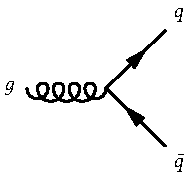
\includegraphics[width=0.7\textwidth]{gluon_quark_vertex}
		\caption{\label{fig:gluon_quark_vertex}}
	\end{subfigure}%
	\begin{subfigure}[b]{0.33\linewidth}
		\centering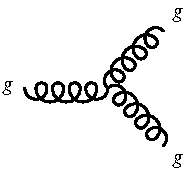
\includegraphics[width=0.7\textwidth]{gluon_vertex}
		\caption{\label{fig:gluon_vertex}}
	\end{subfigure}	
	\begin{subfigure}[b]{0.33\linewidth}
		\centering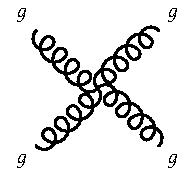
\includegraphics[width=0.7\textwidth]{gluon_quartic_vertex}
		\caption{\label{fig:gluon_quartic_vertix}}
	\end{subfigure}
	\caption{Possible vertices in QCD.}
	\label{fig:qcd_vertices}
\end{figure}

\subsubsection{Electroweak interaction}
\label{sec:ewk_interaction}

During the 1960s, Glashow, Weinberg and Salam~\cite{GLASHOW1961579,PhysRevLett.19.1264,Salam1959} developed a unified theory of the electromagnetic and weak interactions, based on the $SU(2)_\mathrm{L}\otimes U(1)_Y$ symmetry group. Known already experimentally from the Wu experiment`\cite{PhysRev.105.1413} in 1956, weak interaction violates parity, \ie the symmetry transformations have to act differently on the left-handed and right-handed fermion fields. The left- and right-handed components of a fermion field can be projected out using
\begin{equation}
	\psi_\mathrm{L} = \frac{1-\gamma^5}{2}\psi , \ \ \qquad 	\psi_\mathrm{R} = \frac{1+\gamma^5}{2}\psi,
\end{equation}
with $\gamma^5 = i\gamma^0\gamma^1\gamma^2\gamma^3$. As the weak interaction only acts on left-handed fermions, they can be ordered as $SU(2)$ doublets
\begin{equation}
	\begin{pmatrix}
		\nu_e \\
		e
	\end{pmatrix}_\mathrm{L},
	\quad
	\begin{pmatrix}
		u \\
		d
	\end{pmatrix}_\mathrm{L},
	\qquad
	\begin{pmatrix}
		\nu_\mu \\
		\mu
	\end{pmatrix}_\mathrm{L},
	\quad
	\begin{pmatrix}
		c \\
		s
	\end{pmatrix}_\mathrm{L},
	\qquad
	\begin{pmatrix}
		\nu_\tau \\
		\tau
	\end{pmatrix}_\mathrm{L},
	\quad
	\begin{pmatrix}
		t \\
		b
	\end{pmatrix}_\mathrm{L}.
\end{equation} 
The quantum number associated with $SU(2)$ symmetry transformations is called weak isospin $I$ with third component $I_3$. Fermion doublets have $I=1/2$, with the upper component having $I_3 = 1/2$ and the lower component $I_3=-1/2$. Right-handed fermion fields have $I=0$, \ie are singlet states in weak isospin space
\begin{equation}
	e_\mathrm{R},u_\mathrm{R},d_\mathrm{R}, \qquad \mu_\mathrm{R},c_\mathrm{R},s_\mathrm{R}, \qquad \tau_\mathrm{R},t_\mathrm{R},b_\mathrm{R}, 
\end{equation}
and thus do not couple to the weak interaction. In the electroweak theory, neutrinos are assumed to be strictly massless, therefore no right-handed neutrino singlets exist. 

The fermion doublets can be written in a free Lagrangian similar to \cref{eq:dirac_lagrangian,eq:free_lagrangian}
\begin{equation}
	\Lagr = \bar{\psi}_\mathrm{L}i\gamma^\mu\partial_\mu\psi_\mathrm{L},
\end{equation}
with one crucial difference---the omission of the fermion masses. As $\bar{\psi}\psi = \bar{\psi}_\mathrm{L}\psi_\mathrm{R} + \bar{\psi}_\mathrm{R}\psi_\mathrm{L}$, mass terms would mix left- and right-handed terms and break gauge invariance. \Cref{sec:ssb} will illustrate how fermion masses will instead be generated in the electroweak theory. For left-handed fermion fields, local $SU(2)_\mathrm{L}$ transformations can be written as
\begin{equation}
	\psi_\mathrm{L} \rightarrow \mathrm{exp}\left(ig_2\alpha^a\frac{\sigma^a}{2}\right)\psi_\mathrm{L},
\end{equation}  
where $g_2$ is the coupling constant, $\alpha^a$ with $a=1,2,3$ are real parameters and the Pauli matrices $\sigma^a$ are the generators of $SU(2)_\mathrm{L}$. By introducing the covariant derivative $\codiff_\mu = \partial_\mu + ig_2\frac{\sigma^a}{2}W^a_\mu$ and including the usual kinetic term for the gauge fields, the Lagrangian becomes invariant under $SU(2)_\mathrm{L}$ transformations and reads
\begin{equation}
	\Lagr = \bar{\psi}_\mathrm{L}i\gamma^\mu\codiff_\mu\psi_\mathrm{L} - \frac{1}{4}W^a_{\mu\nu}W^{\mu\nu,a},
\end{equation}
with the gauge field strength tensors $W^a_{\mu\nu} = \partial_\mu W^a_\nu - \partial_\nu W^a_\mu + g_2 \epsilon^{abc}W^b_\mu W^c_\nu$ where $\epsilon^{abc}$ are the structure constants. As previously in the case of QCD, the non-Abelian structure of the symmetry group causes self-interactions of the gauge fields.

In order to include electromagnetic interactions, the weak isospin group is extended with the $U(1)_Y$, corresponding to the multiplication of a phase factor $e^{i\alpha\frac{Y}{2}}$ to each of the preceding doublets and singlets. Here, $Y$ is the weak hypercharge as given by the Gell-Mann--Nishijima relation~\cite{Gell-Mann1956,10.1143/PTP.13.285,10.1143/PTP.10.581}
\begin{equation}
	Q = I_3 + \frac{Y}{2},
	\label{eq:gell-mann-nishijima}
\end{equation}
with $Q$ the electric charge. The electromagnetic group $U(1)_\mathrm{em}$ as a subgroup of the combined electroweak gauge group.

By modifying the covariant derivative to include a $U(1)_Y$ gauge field and ensuring that $U(1)_Y$ acts the same on left- and on right-handed fermions it becomes $\codiff_\mu = \partial_\mu + ig_2\frac{\sigma^a}{2}W^a_\mu + ig_1\frac{Y}{2}B_\mu$ for left-handed fermions and $\codiff_\mu = \partial_\mu + ig_1\frac{Y}{2}B_\mu$ for right-handed fermions. Then the full electroweak Lagrangian reads
\begin{equation}
\begin{split}
	\Lagr_\mathrm{electroweak} = & \sum_j^6{\bar{\psi}_\mathrm{L}^j i \gamma^\mu \left(\partial_\mu -ig_2\frac{\sigma^a}{2} W^a_\mu + ig_1 \frac{Y}{2} B_\mu \right) \psi^j_\mathrm{L}} \\
	& + \sum_j^9{\bar{\psi}_\mathrm{R}^j i \gamma^\mu \left(\partial_\mu + ig_1 \frac{Y}{2} B_\mu \right) \psi^j_\mathrm{R}}
\end{split}
\end{equation}
where $B_{\mu\nu} = \partial_\mu B_\nu - \partial_\nu B_\mu$. 

\subsubsection{Spontaneous symmetry breaking}
\label{sec:ssb}

\nomenclature[z-VEV]{VEV}{Vacuum expectation value}


In the electroweak theory a total of three vector fields $W^a_\mu$ and one vector field $B_\mu$ are associated with the gauge groups $SU(2)_\mathrm{L}$ and $U(1)_Y$, respectively. As has been shown explicitly through the example of QED in \cref{sec:gauge_principle}, the gauge fields need to be massless for the resulting Lagrangian to be gauge invariant under the respective symmetry group. In addition, the electroweak symmetry group does not allow for fermion masses. Both gauge bosons of the weak interaction and the fermion are however manifestly massive, hence the electroweak symmetry has to be broken in the SM.

This spontaneous symmetry breaking is achieved through the Brout-Englert-Higgs   mechanism~\cite{PhysRevLett.13.321,PhysRevLett.13.508,PhysRev.145.1156}. In the SM, an isospin doublet of complex scalar fields, called Higgs doublet, is introduced
\begin{equation}
	\Phi(x) = \begin{pmatrix}
		\phi^+(x) \\
		\phi^0(x)
	\end{pmatrix}.
\end{equation}
The Higgs doublet has hypercharge $Y=1$, hence according to \cref{eq:gell-mann-nishijima}, $\phi^+$ has electric charge +1 while $\phi^0$ is electrically neutral. With the covariant derivative introduced in \cref{sec:ewk_interaction}, the Higgs doublet gets an associated part in the SM Lagrangian reading
\begin{equation}
	\Lagr_\mathrm{H} = (\codiff_\mu\Phi)^\dagger(\codiff^\mu\Phi) - V(\Phi),
\end{equation}
where $V(\Phi)$ is a gauge invariant potential
\begin{equation}
	V(\Phi) = -\mu^2\Phi^\dagger\Phi + \frac{\lambda}{4}(\Phi^\dagger\Phi)^2.
	\label{eq:higgs_potential}
\end{equation}
For positive and real parameters $\mu^2$ and $\lambda$, this potential has the form of a \textit{Mexican hat} and an infinite number of minima for field configurations with $\Phi^\dagger\Phi=2\mu^2/\lambda$. In the vacuum, \ie in the ground state of the theory with minimal potential energy of the field, one of these minima is chosen such that the Higgs  receives a vacuum expectation value (VEV)
\begin{equation}
	\braket{\Phi} = \frac{1}{\sqrt{2}}\begin{pmatrix}
		0 \\
		v
	\end{pmatrix} \qquad \textrm{with} \quad v = \frac{2\mu}{\sqrt{\lambda}} \approx \SI{246}{\GeV}.
	\label{eq:higgs_vev}
\end{equation}
This is neither invariant under a $SU(2)_\mathrm{L}$ transformation of the form $U = \mathrm{exp}(i\alpha^a\frac{\sigma^a}{2})$, nor under a $U(1)_Y$ transformation of the form $\mathrm{exp}(i\alpha\frac{Y}{2})$, therefore the electroweak gauge symmetry is spontaneously broken; the Lagrangian has a symmetry that the vacuum does not have. It is worth noting that the $U(1)_\mathrm{em}$ gauge symmetry is not broken as the VEV of $\phi^+$ vanishes and $\phi^0$ is invariant under $U(1)_\mathrm{em}$.

The Higgs doublet can be expressed as excitations around the ground state
\begin{equation}
	\Phi(x) = \frac{1}{\sqrt{2}} \begin{pmatrix}
		\phi_1(x)+i\phi_2(x) \\
		v + H(x) + i\chi(x)
	\end{pmatrix},
	\label{eq:higgs_expansion}
\end{equation}
where $H$, $\chi$, $\phi_1$ and $\phi_2$ are real scalar fields with vanishing VEV. The Higgs potential can then be written as
\begin{equation}
	V = \mu^2H^2 + \frac{\mu^2}{v} H (H^2 + \chi^2 + \phi_1^2+\phi_2^2)+ \frac{\mu^2}{4v^2}(H^2 + \chi^2 + \phi_1^2 + \phi_2^2),
\end{equation}
where only $H$ gets a mass term, thus describing an electrically neutral scalar particle with mass $m_H = \sqrt{2}\mu$. The remaining scalar fields remain massless, in accordance with the Nambu-Goldstone theorem~\cite{Nambu:1960tm,Goldstone:1961eq}, stating that every spontaneously broken continuous symmetry generates a massless Goldstone boson. These bosons are unphysical and can be gauged away through a $SU(2)_\mathrm{L}$ transformation, such that the expansion around the vacuum from \cref{eq:higgs_expansion} involves only the physical scalar $H(x)$
\begin{equation}
	\Phi(x) = \frac{1}{\sqrt{2}} \begin{pmatrix}
		0 \\
		v + H(x)
	\end{pmatrix}.	
\end{equation}
\begin{figure}
	\centering
	\begin{subfigure}[b]{0.33\linewidth}
		\centering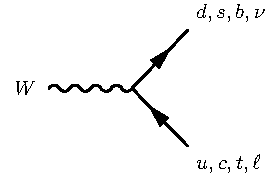
\includegraphics[width=0.8\textwidth]{w_fermion_vertex}
		\caption{\label{fig:w_fermion_vertex}}
	\end{subfigure}%
	\begin{subfigure}[b]{0.33\linewidth}
		\centering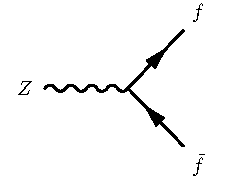
\includegraphics[width=0.8\textwidth]{z_fermion_vertex}
		\caption{\label{fig:z_fermion_vertex}}
	\end{subfigure}	
	\begin{subfigure}[b]{0.33\linewidth}
		\centering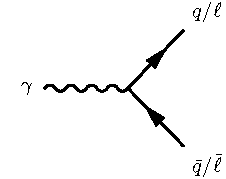
\includegraphics[width=0.8\textwidth]{gamma_fermion_vertex}
		\caption{\label{fig:gamma_fermion_vertex}}
	\end{subfigure}
	\begin{subfigure}[b]{0.33\linewidth}
		\centering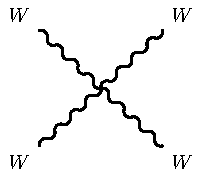
\includegraphics[width=0.7\textwidth]{w_boson_quartic_vertex}
		\caption{\label{fig:w_boson_quartic_vertex}}
	\end{subfigure}%
	\begin{subfigure}[b]{0.33\linewidth}
		\centering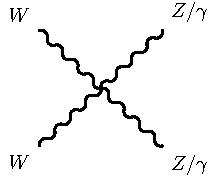
\includegraphics[width=0.7\textwidth]{wz_boson_quartic_vertex}
		\caption{\label{fig:wz_boson_quartic_vertex}}
	\end{subfigure}	
	\begin{subfigure}[b]{0.33\linewidth}
		\centering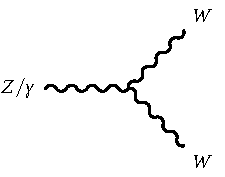
\includegraphics[width=0.7\textwidth]{w_boson_cubic_vertex}
		\caption{\label{fig:w_boson_cubic_vertex}}
	\end{subfigure}
	\caption{Possible vertices in the electroweak interaction.}
	\label{fig:ewk_vertices}
\end{figure}
The gauge transformation bringing \cref{eq:higgs_expansion} into the above form is called the \textit{unitary gauge}. In this gauge, the Higgs potential from \cref{eq:higgs_potential} has the form
\begin{equation}
	V = \frac{m_H^2}{2} H^2 + \frac{m_H^2}{2v} H^3 + \frac{m_H^2}{8v^2} H^4,
\end{equation}
containing cubic and quartic self-interactions of the Higgs field proportional to $m^2_H$. Inserting the excitation around the vacuum state in the kinetic term of the $\Lagr_\mathrm{H}$ yields mass terms for the vector bosons
\begin{equation}
	\Lagr_\mathrm{H} \propto \frac{v^2}{8}g^2_2\left(W_\mu^1W^{1,\mu} + W_\mu^2W^{2,\mu}\right) + \frac{v^2}{8} \begin{pmatrix}
		W^3_\mu & B_\mu
	\end{pmatrix}
	\begin{pmatrix}
		g_2^2 & g_1g_2   \\
		g_1g_2 & g_1^2
	\end{pmatrix}
	\begin{pmatrix}
		W^{3,\mu} \\
		B^\mu
	\end{pmatrix},
\end{equation}
Instead of expressing the Lagrangian in terms of the fields $W^a_\mu$ and $B_\mu$ that make the original gauge invariance manifest, it can also be written in terms of the \textit{physical} fields that correspond to the physical $W^\pm$, $Z$ and $\gamma$ bosons in the electroweak theory
\begin{align*}
	W^\pm_\mu 	& = \frac{1}{\sqrt{2}}(W^1_\mu\mp i W^2_\mu) 				& \textrm{with} \quad m_W  & = \frac{g_2}{2}v, \\
	Z_\mu 		& = \frac{1}{\sqrt{g_1^2+g_2^2}}(g_2W^3_\mu - g_1 B_\mu) 	& \textrm{with} \quad m_Z  & = \frac{\sqrt{g_1^2+g_2^2}}{2}v, \\
	A_\mu 		& = \frac{1}{\sqrt{g_1^2+g_2^2}}(g_1W^3_\mu + g_2 B_\mu) 	& \textrm{with} \quad m_A  & = 0.
\end{align*}
It is worth noting, that the massless photon field $A_\mu$ associated with the electromagnetic $U(1)_\mathrm{em}$ gauge symmetry is automatically recovered. All possible vertices between fermions and the physical electroweak gauge bosons are shown in \cref{fig:ewk_vertices} The change of basis from $(W^3_\mu, B_\mu)$ to $(Z_\mu,A_\mu)$~\cite{Peskin:1995ev} can also be written as a basis rotation with the weak mixing angle $\theta_W$
\begin{equation}
	\begin{pmatrix}
		Z_\mu \\
		A_\mu
	\end{pmatrix} =
	\begin{pmatrix}
		\cos{\theta_W} & \sin{\theta_W} \\
		- \sin{\theta_W} & \cos{\theta_W}
	\end{pmatrix}
	\begin{pmatrix}
		W^3_\mu \\
		B_\mu
	\end{pmatrix} \qquad \textrm{with } \cos{\theta_W} = \frac{g_2}{\sqrt{g_1^2 + g_2^2}} = \frac{m_W}{m_Z}.
\end{equation}

In the SM, not only the $W^\pm$ and $Z$ bosons but also fermions gain their masses through spontaneous breaking of the electroweak gauge symmetry. Fermion fields gain masses through gauge-invariant Yukawa interactions with the Higgs field. For one fermion generation, the respective Yukawa terms in the Lagrangian are
\begin{equation}
	\Lagr_\mathrm{Yukawa,gen} = - \lambda_\ell \bar{L}_\mathrm{L}\Phi\ell_\mathrm{R} - \lambda_d \bar{Q}_\mathrm{L}\Phi d_\mathrm{R} - \lambda_u \bar{Q}_\mathrm{L} \Phi^\dagger u_\mathrm{R} + \mathrm{h.c.},
\end{equation}
where $\lambda_f$ with $f = \ell,d,u$ are the dimensionless Yukawa couplings and $L_\mathrm{L} = (\nu_\mathrm{L},\ell_\mathrm{L})^T$ and $Q_\mathrm{L} = (u_\mathrm{L},d_\mathrm{L})^T$ are the left-handed lepton and quark doublets, respectively. The VEV of the Higgs field then gives rise to fermion mass terms in the Lagrangian, which, in the unitary gauge, reads for a single fermion generation
\begin{equation}
 	\Lagr_\mathrm{Yukawa, gen} = - \sum_{f=\ell,d,u}{\left(m_f\bar{\psi}_f\psi_f + \frac{m_f}{v}H\bar{\psi}_f\psi_f\right)} \qquad \textrm{with} \quad m_f = \frac{1}{\sqrt{2}}\lambda_f v.
\end{equation}
When introducing all three fermion generations, additional Yukawa terms mixing fermions of different generations appear in the Lagrangian. The terms involving quark fields can be parametrised using the Cabibbo–Kobayashi–Maskaw (CKM) matrix $V_\mathrm{CKM}$~\cite{PhysRevLett.10.531,CKM:1973fv}, quantifying the transition probability between quark generations. Since no right-handed neutrinos exist in the SM, no generation mixing in the lepton sector occurs and hence no neutrino mass terms are allowed in the SM. Neutrino oscillations have however been observed experimentally, thus at least one massive neutrino generation needs to exist. Their mixing can then be described with the Pontecorvo-Maki-Nakagawa-Sakata (PMNS) matrix~\cite{PMNS:1962mu}, allowing neutrinos to acquire mass \eg through the see-saw mechanism~\cite{Brdar:2019iem}.
 
\subsection{Renormalisation and divergencies}
\label{ch:renormalisation}

\begin{figure}
	\centering
	\begin{subfigure}[b]{0.33\linewidth}
		\centering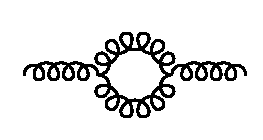
\includegraphics[width=0.85\textwidth]{gluon_loop}
		\caption{\label{fig:gluon_loop}}
	\end{subfigure}%
	\begin{subfigure}[b]{0.33\linewidth}
		\centering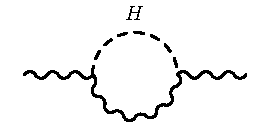
\includegraphics[width=0.85\textwidth]{wz_propagator}
		\caption{\label{fig:wz_propagator}}
	\end{subfigure}	
	\begin{subfigure}[b]{0.33\linewidth}
		\centering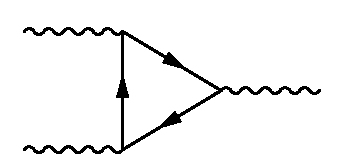
\includegraphics[width=0.85\textwidth]{cubic_vertex}
		\caption{\label{fig:cubic_vertex}}
	\end{subfigure}
	\caption{Examples of loops corrections to (a) the gluon propagator, (b) the $W$ or $Z$ propagator and (c) the cubic gauge boson vertex.}\label{fig:loop_corrections}
\end{figure}

At lowest order in the perturbative expansion, the momenta of the internal lines in the Feynman diagrams are fixed by the external particles. For higher orders where the diagrams involve loops, the momenta of the internal lines need to be integrated over as they are not fixed by energy-momentum conservation. Some examples of loop corrections to propagators and vertices are shown in \cref{fig:loop_corrections}. As each vertex in the Feynman diagrams is associated with a coupling constant that is usually smaller than 1 (apart from the non-perturbative regime of QCD), higher orders in the perturbative expansion contribute less and less to the total amplitude of the full expansion.

The momentum integrals in loop corrections however lead to \textit{ultraviolet divergencies} for large momenta. In order to eliminate the divergencies, the integrals have to be \textit{regularised}, \eg by applying a cut-off scale $\Lambda$ or calculating the integrals in a number $D = 4-\epsilon$ of dimensions where they converge. The potential divergencies are then absorbed in parameters of the Lagrangian, such as coupling constants and masses, after which the regulator is removed (\eg $\epsilon\rightarrow 0$) again and a \textit{renormalisation} procedure is applied, replacing the bare parameter values with the physical, measured values. Renormalisation effectively absorbs the effects of quantum fluctuations acting on much smaller scales than the scale of the given problem in the parameters of the theory.
\improvement{Mass dimension needs to be < 4}
As Veltmann and t'Hooft~\cite{THOOFT1972189,THOOFT1971173} have shown in the early 1970s, all Yang-Mills theories with massive gauge fields are renormalizable, making the SM as a whole a renormalizable theory.  

\section{Supersymmetry}

Among the properties a quantum field theory might possess to make it more mathematically tractable, one specific higher symmetry reveals particularly far-reaching implications; a symmetry relating fermions and bosons, known as \textit{supersymmetry} (SUSY). The following section introduces the basic concepts, a promising class of theories that turns out solving some of the shortcomings of the SM. 

First, a motivation for the need of SUSY is given by highlighting some of the open questions of the SM, followed by an introduction to the mathematical description and phenomenological consequences of supersymmetric theories. This section is intended to highlight the most important concepts and relations, a complete and detailed introduction to SUSY can \eg be found in~\cite{Martin:1997ns}.

\subsection{Shortcomings of the SM}

Although the SM is a wildly successful theory able to predict and describe the interactions between elementary particles with unprecedented precision, there are still phenomena in nature that cannot be suitable understood with the SM. Those limitations and open questions are the reason for numerous searches looking for new physics beyond the Standard Model (BSM). Some of these open questions are described in the following. 

\subsubsection{Dark Matter}

The existence of Dark Matter (DM), \ie non-luminous and non-absorbing matter is nowadays well established~\cite{pdg2020}. Some of the earliest hints for the existence of DM came from the observation that the rotation curves of luminous objects were not consistent with the expected velocities based on the gravitational attraction of the visible objects around them. Zwicky already postulated in 1933 the existence of DM~\cite{Zwicky:437297} based on rotation curves of galaxies in the Coma cluster. In 1970, Rubin measured rotation curves of spiral galaxies~\cite{Rubin:1970zza}, revealing again a significant disagreement with the theoretically expected curves given the visible matter in the galaxies. Based on Newtonian dynamics, the circular velocity of stars outside the bulge of galaxies is expected to fall off with increasing radius as $v(r) \propto 1/\sqrt{r}$~\cite{Bertone:2004pz}. Rubin's observations showed however that the velocities of stars outside the bulge stay approximately constant, strongly suggesting the existence of a non-luminous (or \textit{dark}) halo around the galaxies. Surveys of galaxy clusters and obervations of gravitational lensing effects observed in \eg the bullet cluster~\cite{Clowe:2006eq} or the Abell 1689 cluster~\cite{Taylor:1998uk} have since then further consolidated the existence of large accumulations of non-luminous mass in the universe.

The anisotropies in cosmic microwave background (CMB), studied by the COBE~\cite{Bennett:1996ce,COBE}, WMAP~\cite{WMAP2,WMAP1} and Planck missions~\cite{Planck} are very well described by the Lambda Cold Dark Matter model ($\mathrm{\Lambda CDM}$)~\cite{Liddle:1976476}, which includes a density for cold dark matter. Planck's latest results~\cite{Aghanim:2018eyx} suggest that the matter density of the universe is $\Omega_m = 0.3111\pm 0.0056$\footnote{The remaining $\sim 69\%$ are taken up by \textit{dark energy}, whose nature is still an open question.} and that ordinary baryonic matter only takes up $\sim 4.9\%$ of the universe, while DM accounts to $\sim 26.1\%$.

Candidates for non-baryonic DM need to satisfy certain conditions: they have to be stable on cosmological timescales (otherwise they would have decayed by now), they have to couple only very weakly to the electromagnet interaction (otherwise they would be luminous matter) and they have to have the right relic density. Analyses of structure formations in the Universe have furthermore shown that most DM should have been \textit{cold}, \ie non-relativistic at the beginning of galaxy formation~\cite{Bertone:2004pz}. Candidates for DM particles are \eg sterile neutrinos, axions, primordial black holes, or weakly interacting massive particles (WIMPs).

In the SM, the only DM candidate particle is the neutrino. Given the upper limits on the neutrino masses, an upper bound on their relic density can be computed, revealing that neutrinos are simply not abundant enough to be a dominant component of DM~\cite{Bertone:2004pz}. Many BSM theories naturally predict new WIMPs with masses in the GeV to TeV range. In many SUSY models with exact R-parity conservation (see \cref{sec:rparity}), the lightest supersymmetric particle is neutral and stable and might indeed be an ideal candidate for DM.

\subsubsection{Unification of forces}

\begin{figure}
\floatbox[{\capbeside\thisfloatsetup{capbesideposition={right,center},capbesidewidth=0.4\textwidth}}]{figure}[\FBwidth]
{\caption{Evolution of the inverse coupling constants in the SM (dashed lines) and the MSSM (solid lines) in function of the energy scale $Q$. In the MSSM, the masses of the supersymmetric particles are treated as common threshold varied between $\SI{750}{\GeV}$ and $\SI{2.5}{\TeV}$. Figure taken from~\cite{Martin:1997ns}.}\label{fig:unification_forces}}
{\includegraphics[width=0.5\textwidth]{unification}}
\end{figure}

Apart from the non-perturbative low-energy behaviour of QCD, the SM as a $SU(3)_C\otimes SU(2)_\mathrm{L}\otimes U(1)_Y$ gauge theory apparently gives a complete picture of nature up to the energy scale probed with today's accelerators. However, some peculiar aspects of the SM hint to a more fundamental theory. A prominent example is the question why the electric charges of the electrons and the charges of the quarks of the protons and neutrons in the nuclei exactly cancel, making for electrically neutral atoms~\cite{Brock:1354959}. Or in other words: why are the charges of all observed particles simple multiples of the fundamental charge?

An explanation to many of these peculiarities comes naturally when describing the SM as a unified theory with a single non-Abelian gauge group, usually taken to be $SU(5)$~\cite{PhysRevLett.32.438}. The larger symmetry group with a single coupling constant is then thought to be spontaneously broken at very high energy, such that the known SM interactions are recovered at lower energies. In such a grand unified theory (GUT), the particles in the SM are arranged in anomaly-free \improvement{explain anomaly cancellations} irreducible representations of the gauge group, thereby \eg naturally ensuring the fractional charges of quarks~\cite{Peskin:1995ev}.

In the SM, the coupling constants run towards each other with increasing energy scale, but never exactly meet. In the Minimal Supersymmetric Standard Model (MSSM) with supersymmetric particles at the TeV scale the running couplings meet within their current uncertainties. \Cref{fig:unification_forces} shows the running of the coupling constants in both the SM and the MSSM.

\subsubsection{The Hierarchy Problem}

As the SM is a renormalizable gauge theory, finite results are obtained for all higher-order loop corrections, making the SM a theory that is well-defined up to infinite energies. In renormalisation terms, this means that the cut-off scale $\Lambda$ is theoretically allowed to go to infinity. It is however clear, that the SM cannot be a complete theory of nature and that at some unknown high-energy scale $\Lambda$, \textit{new physics} has to appear. At the very least, a new theoretical framework becomes necessary at the Planck scale $M_P \approx \SI{e18}{\GeV}$ ~\cite{Martin:1997ns}, where quantum gravitational effects can no longer be ignored.

The mass parameters of fermions and massive vector bosons are protected from large quantum corrections by chiral symmetry and gauge symmetry, respectively~\cite{Aitchison:2007fn}. The mass parameter of the scalar Higgs field, on the other hand, gets loop corrections proportional at least to the scale at which new physics sets in. The coupling of the Higgs field to a fermion $f$ with mass $m_f$, depicted in \cref{fig:fermion_loop}, yields a one-loop correction term to the Higgs square mass~\cite{Martin:1997ns} given by
\begin{align}
	\Delta m_H^2 = -\frac{\lvert\lambda_f\rvert^2}{8\pi^2} \Lambda^2 + \dots\, .
	\label{eq:fermion_correction}
\end{align}
Thus, in order to obtain the relatively low value of the Higgs mass in the order of $\SI{e2}{\GeV}$, the quantum corrections to the bare Higgs parameter have to be tuned in such a way that they almost cancel.  Hence, if there is \textit{any} scale of new physics even only several orders of magnitude higher than the electroweak scale, the large quantum corrections to the Higgs mass immediately lead to a \textit{fine-tuning} problem that is considered to be unnatural.

\begin{figure}
	\centering
	\begin{subfigure}[b]{0.5\linewidth}
		\centering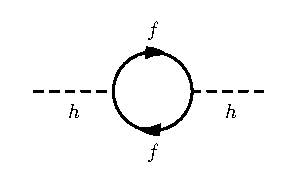
\includegraphics[width=0.75\textwidth]{fermion_loop}
		\caption{\label{fig:fermion_loop}}
	\end{subfigure}%
	\begin{subfigure}[b]{0.5\linewidth}
		\centering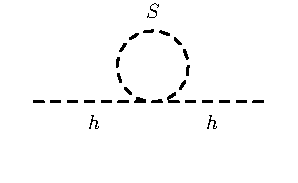
\includegraphics[width=0.75\textwidth]{scalar_loop}
		\caption{\label{fig:scal_loop}}
	\end{subfigure}	
	\caption{A massive fermion \subref{fig:fermion_loop} and a hypothetical massive scalar particle \subref{fig:scal_loop} coupling to the Higgs boson.}\label{fig:loop_corrections_higgs}
\end{figure}

In SUSY, the Higgs mass is automatically protected from the large quantum corrections by the introduction of two complex scalar partners to each SM fermion. The quantum corrections from the a hypothetical heavy complex scalar particle $S$ with mass $m_S$ as in \cref{fig:scal_loop} yields a one-loop correction~\cite{Martin:1997ns} given by 
\begin{align}
	\Delta m_H^2 = \frac{\lambda_S}{16\pi^2}\left[\Lambda^2 + 2m_S^2\log\left(\Lambda/m_S\right)+ \dots\right].
	\label{eq:scalar_correction}
\end{align}
Interestingly, the corrections in \cref{eq:fermion_correction} and \cref{eq:scalar_correction} enter with opposite signs. Thus, if $\lambda_S = \vert\lambda_f\vert^2$, then the large quantum corrections neatly cancel and no excessive fine-tuning is needed. The requirement $\lambda_S = \vert\lambda_f\vert^2$ means that the fermions and their supersymmetric bosonic partners would have same masses. Such particles would have been discovered long ago in particle physics experiments, meaning that SUSY must be a broken symmetry (see \cref{sec:susy_breaking}) such that the supersymmetric particles acquire masses well above their SM partners. 

\subsubsection{Anomalous magnetic moment of the muon}

One of the longest standing disagreements between experiment and theory in the SM is the anomalous magnetic moment of the muon. The magnetic moment of the muon $\vec{\mu}_\mu$ is related to its intrinsic spin $\vec{S}$ through the gyromagnetic ratio $g_\mu$ by
\begin{equation}
	\vec{\mu}_\mu = g_\mu \frac{q}{2m} \vec{S}.
\end{equation}
For a structureless spin-1/2 particle with mass $m$ and charge $q=\pm e$, the gyromagnetic ratio is $g_\mu = 2$~\cite{Bennett:2006fi}. Loop corrections coupling the muon spin to virtual fields cause small deviations, parameterised by the anomalous magnetic moment
\begin{equation}
	a_\mu = \frac{1}{2}(g_\mu-2).
\end{equation}
The anomalous magnetic moment can be precisely measured as well as predicted within the SM, a comparison between experimental data and theoretical prediction thus directly tests the SM at quantum loop level and may hint to effects from new physics in case of discrepancies~\cite{baer_tata_2006}. In the SM, the most dominant contribution to $a_\mu$ comes from QED corrections involving photon and fermion loops. An exemplary diagram is shown in \cref{fig:qed_anomalous_moment}. Weak contributions involving the heavy $W^\pm$, $Z$ and Higgs particles are relatively suppressed due to their mass~\cite{pdg2020}. Although the contributions from QCD are relatively small, they give rise to the main theoretical uncertainties as they are not calculable from first principles~\cite{pdg2020}.

The E821 experiment at Brookhaven National Lab (BNL)~\cite{Bennett:2006fi} has measured the anomalous magnetic moment of the muon and found a deviation from the SM expectation of
\begin{equation}
	\Delta a_\mu = a^\mathrm{exp}_\mu - a^\mathrm{SM}_\mu = 261(63)(48)\times 10^{-11},
\end{equation}
where the numbers in parentheses are the uncertainties from experiment and theory, respectively. This represents a deviation of $3.3\sigma$~\cite{pdg2020} from the SM expectation. 

\begin{figure}
	\centering
	\begin{subfigure}[b]{0.33\linewidth}
		\centering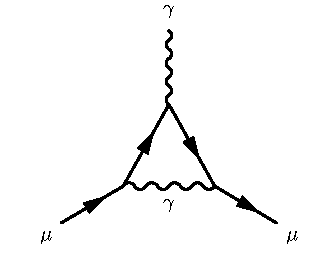
\includegraphics[width=1.0\textwidth]{qed_anomalous_moment}
		\caption{\label{fig:qed_anomalous_moment}}
	\end{subfigure}%
	\begin{subfigure}[b]{0.33\linewidth}
		\centering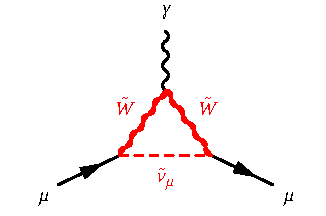
\includegraphics[width=1.0\textwidth]{susy_anomalous_moment_1}
		\caption{\label{fig:susy_anomalous_moment_1}}
	\end{subfigure}%
	\begin{subfigure}[b]{0.33\linewidth}
		\centering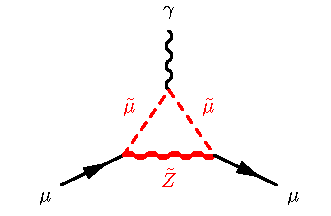
\includegraphics[width=1.0\textwidth]{susy_anomalous_moment_2}
		\caption{\label{fig:susy_anomalous_moment_2}}
	\end{subfigure}	
	\caption{Electromagnetic \subref{fig:qed_anomalous_moment} and supersymmetric \subref{fig:susy_anomalous_moment_1}, \subref{fig:susy_anomalous_moment_2} contributions to $a_\mu$.}\label{fig:loop_corrections_anomalous_moment}
\end{figure}

In SUSY, additional Feynman diagrams exist involving the supersymmetric partners of the muon, the muon neutrino and the electroweak gauge bosons, and thus the measured deviation in $a_\mu$ can easily be accommodated in many supersymmetric models~\cite{Czarnecki:2001pv,Feng:2001tr}. Two exemplary lowest-order diagrams involving supersymmetric particles is shown in \cref{fig:susy_anomalous_moment_1,fig:susy_anomalous_moment_2}.


\subsection{Supersymmetric Algebra}\label{sec:susy_algebra}

A generator of supersymmetric transformations is an anti-commuting spinor $Q$ that turns fermionic states $\ket{f}$ into bosonic states $\ket{b}$ and vice-versa.
\begin{equation}
	Q\ket{f} = \ket{b}, \qquad \qquad \qquad Q\ket{b}=\ket{f}.
\end{equation}
As spinors are complex objects, $Q^\dagger$ is also a symmetry operator. Both $Q$ and $Q^\dagger$ are necessarily fermionic and thus must carry half-integer spin, in the simplest case spin-1/2, meaning that SUSY must be a spacetime symmetry, \ie a Poincaré symmetry. The Coleman-Mandula theorem~\cite{PhysRev.159.1251} dictates that the symmetry group generating a consistent spacetime quantum field theory must be the direct product of the internal symmetry group with the Poincaré group, which in principle rules out the possibility for SUSY. The Haag-Lopuszanski-Sohnius extension~\cite{Haag:1974qh} however states that the only possible way of non-trivially combining internal and spacetime symmetry groups is to use a Lie superalgebra and fermionic spin-1/2 generators. Thus, in order to obey the Haag-Lopuszanski-Sohnius theorem and simultaneously allow for parity-violating interactions, the SUSY generators have to satisfy the following algebra of commutation and anti-commutation relations~\cite{Bustamante:2009us}.
\begin{equation}
\begin{split}
	\{ Q,Q^\dagger \} & \quad = \quad  2\sigma_\mu P^\mu,\\
	\{ Q,Q \} &  \quad = \quad \{ Q^\dagger,Q^\dagger \} = 0, \\
	\left[P^\mu,Q \right] &  \quad = \quad \left[ P^\mu,Q^\dagger \right] = 0, \\
	\{ M^{\mu\nu}, Q \} & \quad = \quad \sigma^{\mu\nu} Q,\\
	\{ M^{\mu\nu},Q^\dagger \} & \quad = \quad \bar{\sigma}^{\mu\nu} Q^\dagger,
  \label{eq:commute}
\end{split}
\end{equation}
where $P^\mu$ is the four-momentum generator of spacetime translations, $\sigma_\mu = (\mathbb{1}_2,\sigma_i)$, $\bar{\sigma}_\mu = (\mathbb{1}_2,-\sigma_i)$ with $i=1,2,3$ and the Pauli matrices $\sigma_i$, and $\sigma^{\mu\nu} = \frac{i}{4}(\sigma^\mu\bar{\sigma}^\nu - \sigma^\nu\bar{\sigma}^\mu)$ as well as $\bar{\sigma}^{\mu\nu} = \frac{i}{4}(\bar{\sigma}^\mu\sigma^\nu - \bar{\sigma}^\nu\sigma^\mu)$. This is the simplest version of SUSY, called $N=1$ symmetry, as it introduces only one pair of generators. Supersymmetric theories with $N\geq 2$ pairs of generators also exist and generally have some theoretical advantages as \eg fewer divergencies in the case of $N=2$ or even no divergencies at all in the case of $N=4$~\cite{Bustamante:2009us}. SUSY models with $N\geq 2$ however do not allow for parity violation and thus fail to describe the physics of the SM, disqualifying them from an experimental point of view~\cite{Bustamante:2009us}.

As both SUSY generators commute with spacetime translations (see \cref{eq:commute}), they also both commute with the squared mass operator $-P^2$. Consequently, particles related by the generators, called \textit{superpartners}, must have equal eigenvalues under $-P^2$, \ie equal masses. Furthermore, the SUSY generators also commute with the gauge transformation generators, hence superpartners must have same electric charge, weak isospin and degrees of freedom in colour space~\cite{Martin:1997ns}.\improvement{Mention link to gravity}


\subsection{Supermultiplets}\label{sec:supermultiplets}

The SM and SUSY particles are arranged in irreducible representations of the SUSY algebra, called \textit{supermultiplets}, that each contain both fermionic and bosonic states, that are superpartners of each other. It can be shown that each supermultiplet has an equal number of fermion and boson degrees of freedom, $n_f = n_b$~\cite{Martin:1997ns}.

The simplest supermultiplet $\Psi$ that can be constructed contains a single Weyl fermion $psi$ and two real scalars, described by a single complex field $phi$, called the \textit{sfermion}. The Weyl fermion has two spin helicity states, hence $n_f=2$, and the complex scalar field has two components with $n_b=1$ each. An additional complex scalar field $F$, called \textit{auxiliary field} and not corresponding to a physical particle, has to be introduced in order to allow the SUSY algebra to close off-shell~\cite{Martin:1997ns}. The supermultiplet $\Psi$ thus reads
\begin{equation}
	\Psi = (\phi,\psi,F).
\end{equation}
Being a pure bookkeeping device, the auxiliary field does not propagate and can be eliminated on-shell with the equations of motion $F=F^*=0$. This supermultiplet is called a \textit{chiral} or \textit{scalar} supermultiplet. 

The next-simplest supermultiplet for which $n_f = n_b$ holds, is the \textit{vector} or \textit{gauge} supermultiplet $\Phi$ containing a spin-1 gauge boson $A^\mu_a$, where $a$ is the index of the gauge group. In order for the theory to be renormalizable, this gauge boson must be massless before spontaneous breaking of the symmetry. As a massless spin-1 boson has two helicity states, $n_b = 2$, the superpartner, called \textit{gaugino}, must be a massless spin-1/2 Weyl fermion $\lambda_a$ with two helicity states, $n_f = 2$~\cite{Martin:1997ns}. An auxiliary real bosonic field $D_a$ is needed in order to balance the degrees of freedom off-shell~\cite{Bustamante:2009us}, completing the supermultiplet to be
\begin{equation}
	\Phi = (\lambda_a,A^\mu_a,D_a).
\end{equation}
 Like the chiral auxiliary field, the gauge auxiliary field does not correspond to a physical particle and can be eliminated on-shell through its equations of motion~\cite{Martin:1997ns}.

\subsection{Supersymmetric Lagrangian}

The simplest supersymmetric model that can be shown to realise the superalgebra is the massless, non-interacting Wess-Zumino model~\cite{WESS197439,Martin:1997ns}, given by 
\begin{equation}
\begin{split}
	\Lagr_\mathrm{free} & = \Lagr_\mathrm{scalar} + \Lagr_\mathrm{fermion} \\
	& = \partial^\mu\phi^*\partial_\mu\phi + i\psi^\dagger\bar{\sigma}^\mu\partial_\mu\psi,
\end{split}
\end{equation}
with a massless complex scalar $\phi$ and a spin-1/2 fermion $\psi$, corresponding to a single chiral supermultiplet. As discussed in \cref{sec:supermultiplets}, in order for this Lagrangian to satisfy the supersymmetry off-shell where the equations of motion cannot be used, an auxiliary complex scalar field $F$ has to be added. For a collection of $i$ chiral supermultiplets, the free Lagrangian reads
\begin{equation}
\begin{split}
	\Lagr_\mathrm{free} & = \Lagr_\mathrm{scalar} + \Lagr_\mathrm{fermion} + \Lagr_\mathrm{aux} \\
	 & = \partial^\mu\phi^{*i}\partial_\mu\phi_i + i\psi^{\dagger i}\bar{\sigma}^\mu\partial_\mu\psi_i + F^*iF_i,
\end{split}
\end{equation} 
where the repreated indices $i$ are summed over. The auxiliary Lagrangian term $\Lagr_\mathrm{aux}$ implies the trivial equations of motion $F = F^* = 0$ which are needed to remove the auxiliary field in the on-shell case. The next step involves adding terms for non-gauge interactions for the chiral supermultiplets  It can be shown that the most general non-gauge interactions for chiral supermultiplets are determined by a holomorphic\footnote{A holomorphic function is a complex-valued function in one or more complex variables that is complex differentiable in a neighbourhood for every point of its domain.} function of the complex scalar fields, called the \textit{superpotential} $W$~\cite{Martin:1997ns, Bustamante:2009us}, which reads
\begin{equation}
	W = \frac{1}{2}m^{ij}\phi_i \phi_j + \frac{1}{6}y^{ijk}\phi_i \phi_j \phi_k,
\end{equation}
with $y^{ij}$ the Yukawa couplings between the scalars and fermions. The superpotential can at most be cubic in order for the final Lagrangian to be renormalizable~\cite{Bustamante:2009us}. The requirement that the interaction part of the Lagrangian be invariant under supersymmetry transformations further defines the potential $V$. The equations of motions of the auxiliary fields $F$ can be written as
\begin{equation}
	F_i = \frac{\partial W(\phi)}{\partial \phi^i} = - W^*_i, \qquad F^{*i} = - \frac{\partial W(\phi)}{\partial \phi_i} = - W^i,
\end{equation} 
which thus yields for the potential $V = W^*_iW^i = F_iF^{*i}$. The full Lagrangian of the Wess-Zumino model with general chiral interactions for $i$ chiral supermultiplets is then given~\cite{Martin:1997ns} by
\begin{equation}
	\Lagr = \partial^\mu\phi^{*i}\partial_\mu\phi_i + i\psi^{\dagger i}\bar{\sigma}^\mu\partial_\mu\psi_i + \frac{1}{2} m^{ij}\psi_i \psi_j + \frac{1}{2} m_{ij}^* \psi^{\dagger i} \psi^{\dagger j} + \frac{1}{2} y^{ijk} \phi_i \psi_j \psi_k + \frac{1}{2} y^*_{ijk} \phi^{*i} \psi^{\dagger j} \psi^{\dagger k} + V.
	\label{eq:wess_zumino_lagrangian}
\end{equation}
The Lagrangian in \cref{eq:wess_zumino_lagrangian} immediately reveals that, as expected by supersymmetry, the masses of the fermions and bosons in the same supermultiplet are identical. In order to incorporate gauge supermultiplets and consider the interactions between fermions and gauge bosons observed in the SM, the usual minimal coupling rule has to be applied, replacing $\partial_\mu$ with $\codiff_\mu$. This leads to equation of motions for the auxiliary fields $D^a$
\begin{equation}
	D^a = -g(\phi^*T^a\phi),
\end{equation}
where $T^a$ are the generators of the gauge group and $g$ is the coupling constant~\cite{Martin:1997ns}. The potential then becomes
\begin{equation}
	V = F^{*i}F_i + \frac{1}{2} \sum_a{D^aD^a} = W^*_iW^i + \frac{1}{2}\sum_a{g^2_a(\phi^*T^a\phi)^2} ,
\end{equation}
where $a$ runs over the gauge groups that in general have different gauge couplings~\cite{Martin:1997ns,Bustamante:2009us}.


 
\subsection{The Minimal Supersymmetric Standard Model}

\subsection{Soft supersymmetry breaking}\label{sec:susy_breaking}

As stated in \cref{sec:susy_algebra}, all superpartners must have same quantum numbers apart from their spin. They especially also should have same masses, however such particles would have been discovered a long time ago and thus SUSY must be broken. The exact breaking mechanism is still an open question.


\subsection{R-parity}\label{sec:rparity}

\subsection{The phenomenological MSSM}

\subsection{Simplified models}